\chapter{はじめに}
ニューラルネットワークモデルの一つであるRecurrent Neural Networks(RNN)は、時系列データの学習に広く用いられる。
入力の順伝播を繰り返す最もシンプルなRNNでは、長時間の入力にわたって逆伝播を計算する中で勾配の値が極端に小さくあるいは大きくなるという問題が発生する。
Long-Short Term Memory(LSTM)\cite{lstm}はゲーティング機構によりこれらの問題に対処した。
また、メモリセルの存在により長時間にわたり情報を保持する能力が向上した。
しかしメモリセルのサイズや複雑さの制限により、多くの情報を長期保持する能力にはまだ限界がある[要出典]。

メモリネットワークはメモリとして利用可能な行列を有し、各時間ステップでの入力情報をメモリに読み書きする能力を学習する。
典型的なメモリネットワークの構造は図\ref{fig:memory_net}
End-To-End Memory Networks\cite{E2E}は入力の埋め込みを外部メモリとして保持することで、入力中の長い時間を隔てた関係を解釈できる。
しかし入力系列の各項目を全て保存する必要があるため、時間方向へのスケーリング能力に課題がある。

\begin{figure}[t]
	\centering
	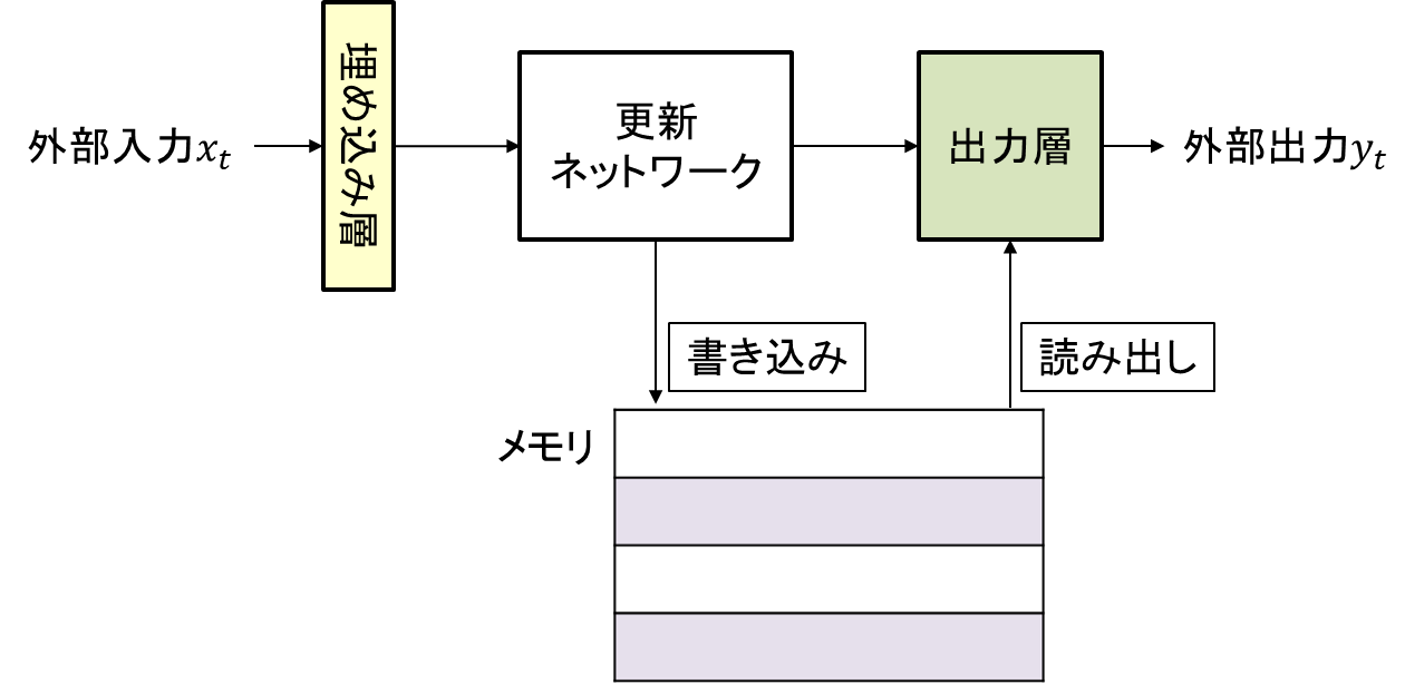
\includegraphics[width=\linewidth]{./figure/img_slide/memory_net.png}
	\caption{典型的なメモリネットワーク}
	\label{fig:memory_net}
\end{figure}

Neural Turing Machine (NTM)\cite{ntm}が有するメモリは固定長であるため、入力の長期化に伴う計算量の増加を回避できる。
メモリスロットの数を超えるサイズの入力系列に対応できるのは、メモリの特定の行を忘却/上書きする能力による。
Differentiable Neural Computer (DNC)\cite{dnc}はNTMの読み出し/書き込み重みの計算部分をより複雑にしたモデルである。
追加モジュールの一つであるusage vectorは、各スロットの使用率を記憶する隠れ状態である。
書き込み重みの算出に利用することで、空いているスロットに優先的に書き込める。
別の追加モジュールであるtemporal link matrixは、スロット間の前後関係を記憶するメモリである。
読み出し重みの計算に利用することで、着目するスロットの前後の時間で書き込まれたスロットも考慮できる。
Convertible Short-Term and Long-Term Memory in DNC (CSLM)\cite{cslm}は、DNCの長期記憶能力をさらに改善する。
メモリの各スロットには重要度が割り振られており、これは学習を通して変化可能である。
重要度の割り当てが低いスロットは忘却されやすく、高いスロットはその逆になる。
これはDNCのメモリがスロット単位で長期記憶と短期記憶に分けられており、その割り当ては適応的かつ学習可能であることを意味する。

これらNTMベースのモデルは学習を通して書き込みの位置や読み出す内容を最適化できる。
しかしメモリの項目間の関係を計算する機構を持たないため、最短経路探索のような入力実体間の関係推論を要求するタスクでの性能に劣る。

関係ネットワークは入力や記憶内の実体間の関係推論能力を持つ。関係の計算はself-attention\cite{transformer}をベースにした手法で行われる。
Relational recurrent neural networks (R-RNN)\cite{rrnn}で提案されたRelational Memory Core(RMC)は、毎時間ステップにおいて入力と全メモリスロット間での関係情報を計算し、その情報でメモリを更新する。
Self-Attentive Associative Memory (SAM)\cite{sam}で提案されたSAM-based Two-memory Model(STM)は、入力を保存する項目メモリと、保存した項目間の関係情報を保存する関係メモリの2種類のメモリを持つ。
項目を忠実に復元することを要求するタスクにおいて、関係メモリのみを持つRMCよりも高い精度を示している。
NTMのように項目がメモリスロット間で区分けされるモデルと異なり、SAMの2つのメモリは分散型のメモリである。
項目メモリは入力のouter productを保存する自己連想記憶、関係メモリは項目メモリから抽出した項目間のouter productを保存する相互連想記憶として実装されており、各入力がメモリ全体に分散するためである。

本論文ではNTMのメモリ構造を保ったまま関係推論モジュールを追加し、メモリ項目間の関係推論能力を追加することを提案する。
関係メモリにはRMCを用いるため、提案ネットワークはNTMを項目メモリ、RMCを関係メモリとして持つ2メモリモデルとなる。
同じ2メモリモデルであるSAMと比較すると、項目メモリが非分散型メモリであり各行で記憶内容が区分けされているある点が異なる。
これにより各入力項目を選択的に忘却・上書きすることが可能になり、R-RNNやSAMのような分散記憶+LSTM方式の忘却よりも高度な忘却が行えると考えられる。
従って長期記憶保持が必要なタスクでより優れた性能を示すことが期待される。
CSLMが各スロットに忘却強度を割り振ったように、読み書き・忘却方式に拡張性・柔軟性があることも利点である。
またこれらのメモリの読み書きはアテンションに由来する説明可能性がある。アテンション係数を可視化することで読み書きした番地を追跡可能である。


この論文の貢献は以下に示す通りである
\\1.NTMに関係推論能力を付与する。このとき関係メモリの入力から一貫性が失われることが予想される。この課題をGATと書き込み頻度ソートの2種類のモジュールにより解決する。
\\2.非分散型のメモリの実装により、分散型メモリよりも長期記憶が必要なタスクに適している。
\\3. 非分散型のメモリにはCSLMに代表されるように拡張性・柔軟性がある。またアテンションを用いる読み書きにより、メモリ操作は説明可能性を持つ。

